\begin{abox}
	Assignment-S03\\
	\vspace{0.5cm}
	 Polarisation and Boundary Condition
	\end{abox}
\begin{enumerate}
	\item $\left. \right. $
	\begin{answer}
		\begin{align*}
		\rho_{\mathrm{b}}&=-\vec{\nabla} \cdot \overrightarrow{\mathrm{P}}=-\frac{1}{\mathrm{r}^{2}} \frac{\partial}{\partial \mathrm{r}}\left(\mathrm{r}^{2} \frac{-\alpha}{\mathrm{r}}\right)=\frac{\alpha}{\mathrm{r}^{2}}\\\text{ and} \sigma_{\mathrm{b}}&=\overrightarrow{\mathrm{P}} \cdot \hat{\mathrm{n}}=\left\{\begin{array}{l}+\overrightarrow{\mathrm{P}} \cdot \hat{\mathrm{r}}=-\frac{\alpha}{\mathrm{R}_{2}}\left(\text { at } \mathrm{r}=\mathrm{R}_{2}\right) \\ -\overrightarrow{\mathrm{P}} \cdot \hat{\mathrm{r}}=\frac{\alpha}{\mathrm{R}_{1}}\left(\text { at } \mathrm{r}=\mathrm{R}_{1}\right)\end{array}\right\}\\
	\text{	For, }\mathrm{R}_{1}<\mathrm{r}<\mathrm{R}_{2} ; \mathrm{Q}_{\mathrm{enc}}&=\left(\frac{\alpha}{\mathrm{R}_{1}}\right) \times 4 \pi \mathrm{R}_{1}^{2}+\int_{\mathrm{R}_{1}}^{\mathrm{r}}\left(\frac{\alpha}{\mathrm{r}^{2}}\right) 4 \pi \mathrm{r}^{2} \mathrm{dr}\\
		\Rightarrow Q_{e n c}&=4 \pi \alpha R_{1}+4 \pi \alpha\left(r-R_{1}\right)=4 \pi \alpha r \Rightarrow \vec{E}\\&=\frac{1}{4 \pi \varepsilon_{0}} \frac{Q_{e n c}}{r^{2}} \Rightarrow \vec{E}=\frac{\alpha}{\varepsilon_{0} r} \hat{r}
		\end{align*}
	\end{answer}
	\item $\left. \right. $
	\begin{answer}
		\begin{align*}
		\vec{E}&=\left\{\begin{array}{ll}0, & \mathrm{r}<\mathrm{R}_{1} \\ \frac{\mathrm{Q}}{4 \pi \varepsilon_{0} \mathrm{Kr}^{2}} \hat{\mathrm{r}}, & \mathrm{R}_{1}<\mathrm{r}<\mathrm{R}_{2} \\ \frac{\mathrm{Q}}{4 \pi \varepsilon_{0} \mathrm{r}^{2}} \hat{\mathrm{r}}, & \mathrm{r}>\mathrm{R}_{2}\end{array}\right.\\
		\text{(a) Polarisation }\vec{P}&=\varepsilon_{0} \chi_{e} \vec{E}=\varepsilon_{0}(K-1) \times \frac{Q}{4 \pi \varepsilon_{o} K r^{2}} \hat{r}=\frac{Q(K-1)}{4 \pi K r^{2}} \hat{r}\\
		\because \varepsilon&=\varepsilon_{0} \varepsilon_{r}=\varepsilon_{0}\left(1+\chi_{e}\right) \Rightarrow \varepsilon_{r}=K=\left(1+\chi_{e}\right) \Rightarrow \chi_{e}=K-1\\
		\text{The surface bound charge}&\text{ density at }r=R_{2}\text{ is }\sigma_{b}=\vec{P} \cdot \hat{n}=\frac{Q(K-1)}{4 \pi K R_{2}^{2}} \hat{r} \cdot(\hat{r})=\frac{Q(K-1)}{4 \pi K R_{2}^{2}}\\
		\rho_{\mathrm{b}}&=-\vec{\nabla} \cdot \overrightarrow{\mathrm{P}}=-\frac{\mathrm{Q}(\mathrm{K}-1)}{4 \pi \mathrm{K}} \vec{\nabla} \cdot\left(\frac{\hat{\mathrm{r}}}{\mathrm{r}^{2}}\right)\\&=-\frac{\mathrm{Q}(\mathrm{K}-1)}{4 \pi \mathrm{K}} 4 \pi \delta^{3}(\mathrm{r})=-\frac{\mathrm{Q}(\mathrm{K}-1)}{\mathrm{K}} \delta^{3}(\mathrm{r})\\
		\text{(b) }\mathrm{W}&=\frac{1}{2} \int_{\text {all space }}(\overrightarrow{\mathrm{D}} \cdot \overrightarrow{\mathrm{E}}) \mathrm{d} \tau\\&=\frac{\varepsilon_{0}}{2} \frac{\mathrm{Q}^{2}}{\left(4 \pi \varepsilon_{0}\right)^{2}}\left\{\varepsilon_{\mathrm{r}} \int_{\mathrm{R}_{1}}^{\mathrm{R}_{2}} \frac{1}{\mathrm{~K}^{2} \mathrm{r}^{4}} 4 \pi \mathrm{r}^{2} \mathrm{dr}+\int_{\mathrm{R}_{2}}^{\infty} \frac{1}{\mathrm{r}^{4}} 4 \pi \mathrm{r}^{2} \mathrm{dr}\right\}\\
		\mathrm{W}&=\frac{\mathrm{Q}^{2}}{8 \pi \varepsilon_{0}}\left\{\left.\frac{1}{\mathrm{~K}}\left(-\frac{1}{\mathrm{r}}\right)\right|_{\mathrm{R}_{1}} ^{\mathrm{R}_{2}}+\left.\left(\frac{-1}{\mathrm{r}}\right)\right|_{\mathrm{R}_{2}} ^{\infty}\right\} \Rightarrow \mathrm{W}\\&=\frac{\mathrm{Q}^{2}}{8 \pi \varepsilon_{0}}\left\{\frac{1}{\mathrm{~K}}\left(\frac{1}{\mathrm{R}_{1}}-\frac{1}{\mathrm{R}_{2}}\right)+\frac{1}{\mathrm{R}_{2}}\right\}
		\end{align*}
	\end{answer}
	\item $\left. \right. $
	\begin{answer}
		\begin{align*}
		\overrightarrow{\mathrm{E}}&=\left\{\begin{array}{ll}0,\quad  \mathrm{r}<\mathrm{R}_{\mathrm{A}} \\ \frac{\mathrm{Q}}{4 \pi \varepsilon(\mathrm{r}) \mathrm{r}^{2}} \hat{\mathrm{r}},\quad  \mathrm{R}_{\mathrm{A}}<\mathrm{r}<\mathrm{R}_{\mathrm{B}} \\ \frac{\mathrm{Q}}{4 \pi \varepsilon_{0} \mathrm{r}^{2}} \hat{\mathrm{r}}, \quad \mathrm{r}>\mathrm{R}_{\mathrm{B}}\end{array}\right.\text{ or }\overrightarrow{\mathrm{E}}=\left\{\begin{array}{ll}0, & \mathrm{r}<\mathrm{R}_{\mathrm{A}} \\ \frac{\mathrm{Q}}{4 \pi \varepsilon_{0} \mathrm{r}^{3}} \hat{\mathrm{r}}, & \mathrm{R}_{\mathrm{A}}<\mathrm{r}<\mathrm{R}_{\mathrm{B}} \because \varepsilon(\mathrm{r})=\varepsilon_{0} \mathrm{r} \\ \frac{\mathrm{Q}}{4 \pi \varepsilon_{0} \mathrm{r}^{2}} \hat{\mathrm{r}}, & \mathrm{r}>\mathrm{R}_{\mathrm{B}}\end{array}\right.\\
		\text{(a) Polarisation }\vec{P}&=\varepsilon_{0} \chi_{e} \vec{E}=\varepsilon_{0}(r-1) \times \frac{Q}{4 \pi \varepsilon_{o} r^{3}} \hat{r}=\frac{Q(r-1)}{4 \pi r^{3}} \hat{r}\\
		\because \varepsilon&=\varepsilon_{0} \varepsilon_{r}=\varepsilon_{0}\left(1+\chi_{e}\right) \Rightarrow\left(1+\chi_{e}\right)=r \Rightarrow \chi_{e}=r-1\\
		\text{The surface bound }&\text{charge density at }r=R_{B}\text{ is }\sigma_{b}=\vec{P} . \hat{n}=\frac{Q\left(R_{B}-1\right)}{4 \pi R_{B}^{3}} \hat{r} .(\hat{r})=\frac{Q\left(R_{B}-1\right)}{4 \pi R_{B}^{3}}\\
		\text{(b) }\mathrm{W}&=\frac{1}{2} \int_{\text {allspace }}(\overrightarrow{\mathrm{D}} \cdot \overrightarrow{\mathrm{E}}) \mathrm{d} \tau=\frac{\varepsilon_{0}}{2} \frac{\mathrm{Q}^{2}}{\left(4 \pi \varepsilon_{0}\right)^{2}}\left\{\int_{\mathrm{R}_{\mathrm{A}}}^{\mathrm{R}_{\mathrm{B}}} \mathrm{r} \frac{1}{\mathrm{r}^{6}} 4 \pi \mathrm{r}^{2} \mathrm{dr}+\int_{\mathrm{R}_{\mathrm{B}}}^{\infty} \frac{1}{\mathrm{r}^{4}} 4 \pi \mathrm{r}^{2} \mathrm{dr}\right\}\\
		\mathrm{W}&=\frac{\mathrm{Q}^{2}}{8 \pi \varepsilon_{0}}\left\{\left.\left(-\frac{1}{2 \mathrm{r}^{2}}\right)\right|_{\mathrm{R}_{\mathrm{A}}} ^{\mathrm{R}_{\mathrm{B}}}+\left.\left(\frac{-1}{\mathrm{r}}\right)\right|_{\mathrm{R}_{\mathrm{B}}} ^{\infty}\right\} \Rightarrow\\ \mathrm{W}&=\frac{\mathrm{Q}^{2}}{8 \pi \varepsilon_{0}}\left\{\frac{1}{2}\left(\frac{1}{\mathrm{R}_{\mathrm{A}}^{2}}-\frac{1}{\mathrm{R}_{\mathrm{B}}^{2}}\right)+\frac{1}{\mathrm{R}_{\mathrm{B}}}\right\}
		\end{align*}
	\end{answer}
	\item $\left. \right. $
	\begin{answer}
		\begin{align*}
		\vec{P}&=k x \hat{x}\\
		\text{Volume charge density }\rho_{b}&=-\vec{\nabla} \cdot \vec{P}=-k
		\intertext{Bound surface charge density on the surface $O A D G O(y=0$ plane $)$}
		\sigma_{b}&=\vec{P} \cdot \hat{n}=k x \hat{x} .(-\hat{y})=0
		\intertext{Bound surface charge density on the surface $\operatorname{EBCFE}(y=l$ plane $)$}
		\sigma_{b}&=\vec{P} \cdot \hat{n}=k x \hat{x} .(+\hat{y})=0
		\intertext{Bound surface charge density on the surface $\operatorname{OGFE} O(x=0$ plane $)$}
		\sigma_{b}&=\vec{P} \cdot \hat{n}=k x \hat{x} .(-\hat{x})=-k x=0
	\intertext{	Bound surface charge density on the surface $A D C B A(x=l$ plane $)$}
		\sigma_{b}&=\vec{P} . \hat{n}=k x \hat{x} .(\hat{x})=k x=k l
	\intertext{	Bound surface charge density on the surface $O A B E O(z=0$ plane $)$}
		\sigma_{b}&=\vec{P} . \hat{n}=k x \hat{x} .(-\hat{z})=0
	\intertext{	Bound surface charge density on the surface $\operatorname{GFCDG}(z=l$ plane $)$}
		\sigma_{b}&=\vec{P} . \hat{n}=k x \hat{x} .(+\hat{z})=0
		\end{align*}
	\end{answer}
	\item $\left. \right. $
	\begin{answer}
		\begin{align*}
	 \text{(a) }\because \vec{P}&=3 \hat{i}+4 \hat{j} \Rightarrow \rho_{b}=-\vec{\nabla} \cdot \vec{P}=0\\
		\text{(b) At }x&=0, \sigma_{b}=\vec{P} \cdot \hat{n}=(3 \hat{i}+4 \hat{j}) \cdot(-\hat{i})=-3 ; \quad\text{ At }x=1, \sigma_{b}=\vec{P} \cdot \hat{n}=(3 \hat{i}+4 \hat{j}) \cdot(\hat{i})=3\\
		\text{(c) At }y&=0, \sigma_{b}=\vec{P} \cdot \hat{n}=(3 \hat{i}+4 \hat{j}) \cdot(-\hat{j})=-4 ; \quad\text{ At }y=1, \sigma_{b}=\vec{P} \cdot \hat{n}=(3 \hat{i}+4 \hat{j}) \cdot(\hat{j})=4
		\end{align*}
	\end{answer}
	\item $\left. \right. $
	\begin{answer}$\left. \right. $
		\begin{figure}[H]
			\centering
			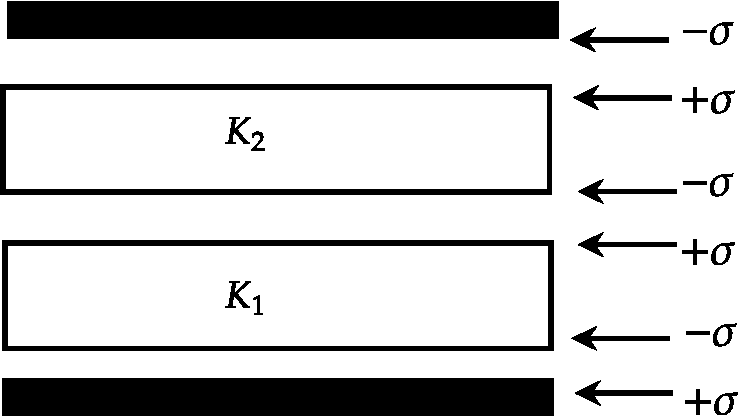
\includegraphics[height=3cm,width=5cm]{Assi-S13}
		\end{figure}
		\begin{align*}
		V&=E_{1} d+E_{2} d=\frac{\sigma}{\varepsilon_{1}} d+\frac{\sigma}{\varepsilon_{2}} d=\frac{\sigma}{K_{1} \varepsilon_{0}} d+\frac{\sigma}{K_{2} \varepsilon_{0}} d\\&=\frac{\sigma d}{\varepsilon_{0}}\left(\frac{1}{K_{1}}+\frac{1}{K_{2}}\right)=\frac{\sigma d}{\varepsilon_{0}}\left(\frac{K_{1}+K_{2}}{K_{1} K_{2}}\right)\\
		\Rightarrow \sigma&=\frac{\varepsilon_{0} V}{d}\left(\frac{K_{1} K_{2}}{K_{1}+K_{2}}\right)\\
		\overrightarrow{P_{1}}&=\varepsilon_{0} \chi_{e} \overrightarrow{E_{1}}=\varepsilon_{0}\left(K_{1}-1\right) \overrightarrow{E_{1}} \Rightarrow \sigma_{1}=\overrightarrow{P_{1}} \cdot \hat{n}\\
		\Rightarrow \sigma_{1}&=\varepsilon_{0}\left(K_{1}-1\right) \times \frac{\sigma}{K_{1} \varepsilon_{0}}\\&=\frac{\left(K_{1}-1\right) \sigma}{K_{1}}=\frac{\left(K_{1}-1\right)}{K_{1}} \frac{\varepsilon_{0} V}{d}\left(\frac{K_{1} K_{2}}{K_{1}+K_{2}}\right)=\frac{K_{2}\left(K_{1}-1\right)}{K_{1}+K_{2}} \frac{\varepsilon_{0} V}{d}\\
		\overrightarrow{P_{2}}&=\varepsilon_{0} \chi_{e} \overrightarrow{E_{2}}=\varepsilon_{0}\left(K_{2}-1\right) \overrightarrow{E_{1}} \Rightarrow \sigma_{2}=\overrightarrow{P_{2}} \cdot \hat{n}\\
		\Rightarrow \sigma_{2}&=\varepsilon_{0}\left(K_{2}-1\right) \times \frac{\sigma}{K_{2} \varepsilon_{0}}=\frac{\left(K_{2}-1\right) \sigma}{K_{2}}=\frac{\left(K_{2}-1\right)}{K_{2}} \frac{\varepsilon_{0} V}{d}\left(\frac{K_{1} K_{2}}{K_{1}+K_{2}}\right)=\frac{K_{1}\left(K_{2}-1\right)}{K_{1}+K_{2}} \frac{\varepsilon_{0} V}{d}\\
		\Rightarrow \sigma&=\sigma_{1}-\sigma_{2}=\frac{K_{2}\left(K_{1}-1\right)}{K_{1}+K_{2}} \frac{\varepsilon_{0} V}{d}-\frac{K_{1}\left(K_{2}-1\right)}{K_{1}+K_{2}} \frac{\varepsilon_{0} V}{d}=\frac{\varepsilon_{0} V}{d\left(K_{1}+K_{2}\right)}\left[K_{2}\left(K_{1}-1\right)-K_{1}\left(K_{2}-1\right)\right]\\
		\Rightarrow \sigma&=\frac{\varepsilon_{0} V}{d} \frac{\left(K_{1}-K_{2}\right)}{\left(K_{1}+K_{2}\right)}
		\end{align*}
	\end{answer}
	\item $\left. \right. $
	\begin{answer}
		\begin{align*}
		\text{(a) }\because E_{1}^{\mathrm{U}}&=E_{2}^{\mathrm{U}} \Rightarrow E_{2}^{\mathrm{U}}=3 \hat{i}-5 \hat{j}\\
		\text{and }\sigma_{f}&=0 \Rightarrow D_{1}^{\perp}=D_{2}^{\perp} \Rightarrow E_{2}^{\perp}=\frac{\varepsilon_{1}}{\varepsilon_{2}} E_{1}^{\perp}=\frac{5}{4}(+4 \hat{k})=5 \hat{k} \Rightarrow \vec{E}_{2}=(3 \hat{i}-5 \hat{j}+5 \hat{k})\\
	\text{	(b) }\vec{D}_{2}&=\varepsilon_{2} \vec{E}_{2}=4 \varepsilon_{0}(3 \hat{i}-5 \hat{j}+5 \hat{k})=\varepsilon_{0}(12 \hat{i}-20 \hat{j}+20 \hat{k})
		\end{align*}
	\end{answer}
	\item $\left. \right. $
	\begin{answer}
		\begin{align*}
		\frac{\tan \theta_{1}}{\tan \theta_{2}}&=\frac{\frac{E_{1}^{\perp}}{E_{1}^{\|}}}{\frac{E_{2}^{\perp}}{E_{2}^{\|}}}=\frac{E_{1}^{\perp}}{E_{2}^{\perp}} \quad\left(\because E_{1}^{\|}=E_{2}^{\|}\right)\\
		D_{1}^{\perp}&=D_{2}^{\perp} \Rightarrow \varepsilon_{1} E_{1}^{\perp}=\varepsilon_{2} E_{2}^{\perp} \Rightarrow \frac{E_{1}^{\perp}}{E_{2}^{\perp}}=\frac{\varepsilon_{2}}{\varepsilon_{1}} \\
		\Rightarrow \frac{\tan \theta_{1}}{\tan \theta_{2}}&=\frac{\varepsilon_{2}}{\varepsilon_{1}} \Rightarrow \varepsilon_{1} \tan \theta_{1}=\varepsilon_{2} \tan \theta_{2}
		\end{align*}
	\end{answer}
	\item $\left. \right. $
	\begin{answer}$\left. \right. $
		\begin{figure}[H]
			\centering
			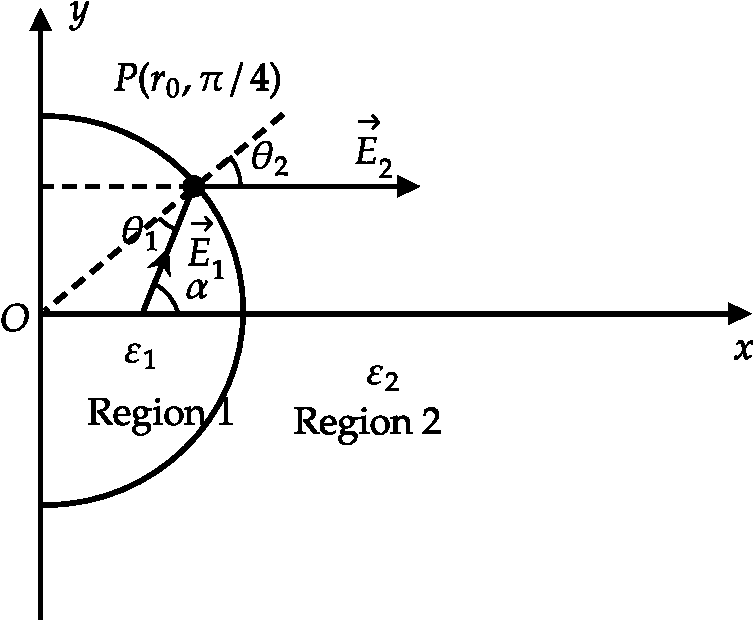
\includegraphics[height=5cm,width=6cm]{Assi-S14}
		\end{figure}
		\begin{align*}
	\because \vec{E}_{1}&=7 \hat{e}_{r}-3 \hat{e}_{\varphi}\\
		\Rightarrow E_{x}&=\left(7 \hat{e}_{r}-3 \hat{e}_{\varphi}\right) \hat{x}=7 \cos 45-3(-\sin 45)=\frac{10}{\sqrt{2}} \\
		\Rightarrow E_{y}&=\left(7 \hat{e}_{r}-3 \hat{e}_{\varphi}\right) \cdot \hat{y}=7 \sin 45-3 \cos 45=\frac{4}{\sqrt{2}} \\
		\text { Thus } \vec{E}_{1} \text { makes an angle } \alpha&=\tan ^{-1}\left(\frac{E_{y}}{E_{x}}\right)=\tan ^{-1}\left(\frac{4}{10}\right)=21.8^{0}\\
		\because \frac{\tan \theta_{2}}{\tan \theta_{1}}&=\frac{\varepsilon_{2}}{\varepsilon_{1}} \Rightarrow \frac{\varepsilon_{2}}{\varepsilon_{1}}=\frac{\tan 45}{\tan 23.2}=2.32 \quad \text{where }\theta_{1}=\alpha-45^{\circ}\text{ and }\theta_{2}=45^{\circ}
		\end{align*}
	\end{answer}
	\item $\left. \right. $
	\begin{answer}
		\begin{align*}
	\sigma&=-\left.\varepsilon_{0} \frac{\partial V}{\partial r}\right|_{r=a}=-\varepsilon_{0}\left[-3 E_{0} \cos \theta-\frac{8 E_{0} a^{3}}{r^{3}} \cos \theta\right]_{r=a}.\\
		\sigma&=-\varepsilon_{0}\left[-3 E_{0} \cos \theta-8 E_{0} \cos \theta\right] \Rightarrow \sigma=11 E_{0} \varepsilon_{0} \cos \theta\\&=11 E_{0} \varepsilon_{0} \cos 60^{\circ}=\frac{11}{2} \varepsilon_{0} E_{0}
		\end{align*}
	\end{answer}
	
\end{enumerate}